\documentclass{report}
\usepackage{graphicx} % Required for inserting images
\usepackage[italian]{babel}
\usepackage{tikz}
\usepackage{hyperref}
\usepackage{amsmath}
\usepackage{xcolor}
\usepackage{float}
\usepackage{soul}
\usepackage{listings} % Per evidenziare il codice

\definecolor{lightgray}{rgb}{0.9,0.9,0.9} % Definizione colore sfondo
\definecolor{darkgreen}{rgb}{0.0, 0.5, 0.0}

\lstset{
    backgroundcolor=\color{lightgray}, % Sfondo grigio
    basicstyle=\ttfamily, % Font monospaziato
    % frame=single, % Bordo attorno al codice
    tabsize=4, % Dimensione tabulazione
    breaklines=true, % Permette di andare a capo automaticamente
    numbers = left,
    numberstyle=\small\color{gray}
}

\title{\huge\textbf{{Controllo delle Query Distribuite}}}
\date{Parte III}

\begin{document}

\maketitle
\tableofcontents
\newpage


\chapter{Introduzione}

Torniamo a preoccuparci del problema di confidenzialità, nel contesto di computazione di 
query distribuite; l'assunzione è che non tutti siano autorizzati a vedere tutti i dati, ma ci 
sono dei vincoli di confidenzialità che devono essere rispettati.

\noindent Lo scenario di riferimento è quello in cui ci sono più sorgenti informative, dove 
da un lato ho l'esigenza di condivisione dei dati (per rispondere alle query), mentre dall'altro 
ho esigenza di confidenzialità perché non è detto che chiunque possa leggere i dati.

\section{Join sovrani}
Questo approccio sfrutta la presenza di un hardware fidato (nel senso che nessuno può vedere 
cosa fa), che può ricevere i dati 
per eseguire le computazioni. Lo scenario è:
\begin{itemize}
    \item si hanno due \textit{data owner} che non si fidano l'uno dell'altro
    \item c'è una terza parte, che ha a disposizione dell'hardware fidato, che esegue la computazione
\end{itemize}

\noindent L'idea è che le parti criptano i dati e li mandano all'hardware, che si occupa di:
\begin{itemize}
    \item decriptare i dati 
    \item eseguire la computazione 
    \item recriptare i dati e darli al client 
\end{itemize}

\noindent Un osservatore potrebbe inferire sulla base del risultato qualcosa, come ad esempio 
sulle dimensioni del risultato o sul tempo richiesto ad eseguire la computazione.

\noindent $\Rightarrow$ l'output deve avere più o meno sempre la stessa dimensione e tempo di computazione, 
per cercare di ridurre l'inferenza

\section{Access patterns}
Cercano di specificare come le fonti informative devono essere accedute.

\noindent Definiamo un \textit{access pattern} con un esempio:
\begin{itemize}
    \item abbiamo 3 relazioni, ciascuna con un access pattern, ovvero dei vincoli di accesso
    \item si ha una lettera per ciasuno attributo delle relazione
    \begin{itemize}
        \item $o$ per output 
        \item $i$ per input 
    \end{itemize}

    \begin{figure}[H]
        \centering
        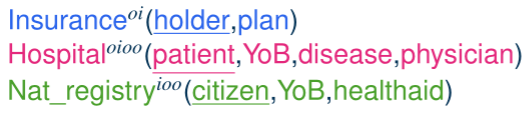
\includegraphics[width=0.6\linewidth]{images/access-pattern.png}
    \end{figure}

    \noindent \textit{per accedere all'attributo "o" mi deve dare l'attributo "i"}; si pongono dei vincoli, 
    l'accesso non è libero
\end{itemize}

\noindent Questa tecnica presenta alcuna svantaggi:
\begin{itemize}
    \item limitata espressione delle limitazioni 
    \item tipicamente ci sono due entità, non un vero scenario distribuito 
    \item può essere difficile da usare nella pratica 
\end{itemize}

\section{Autorizzazioni basate su viste}
La peculiarità di questo approccio è che le restrizioni di accesso dipendono dal contenuto del dato.

\begin{figure}[H]
    \centering
    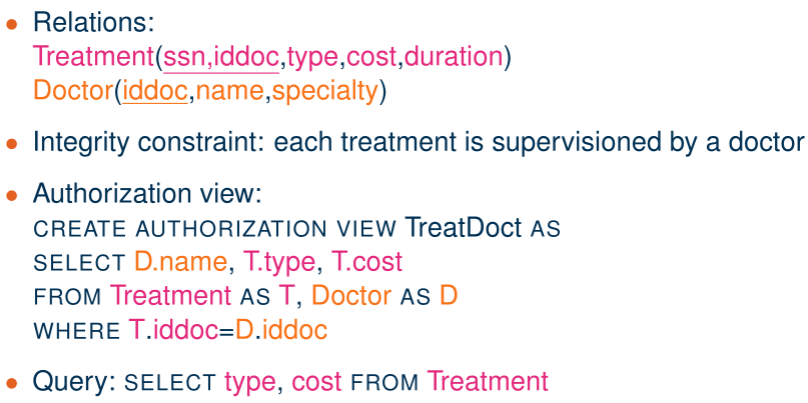
\includegraphics[width=0.8\linewidth]{images/view-auth.png}
\end{figure}

\noindent Verifico se una query può essere eseguita sulla base delle autorizzazioni che 
ho definito; il client scrive la sua query, e il server cerca di rielaborarla 
sulla base delle viste che sono state definite.

\noindent Nel caso in cui una query non possa essere eseguita, ci sono due scenari possibili:
\begin{itemize}
    \item \textit{truman:} ti restituisco un risultato parziale, che corrisponde non alla query che mi hai chiesto ma alla vista che è stata definita (facendotelo 
    passare come completo)
    \item \textit{non-truman:} non ti restituisco nulla e ti dico che non sei autorizzato ad accedere al risultato 
\end{itemize}


\section{Coalition networks}
Ci sono diversi \textit{providers} che si conoscono e che formano delle \textit{coalizioni}; sono 
disposti a condividere le proprie informazioni per un obiettivo comune.

\noindent Ciascun provider ha:
\begin{itemize}
    \item una o più relazioni 
    \item uno o più server
\end{itemize}

\begin{figure}[H]
    \centering
    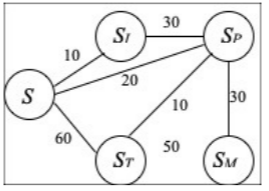
\includegraphics[width=0.4\linewidth]{images/pairwise-auth.png}
\end{figure}

\noindent I server formano una rete, possono comunicare tra di loro; una computazione vuole essere effettuata 
\textbf{minimizzando il costo} (ciascun canale a un costo asssociato) e \textbf{rispettando le restrizioni} 
sul flusso di informazioni (chi può vedere che cosa).


\noindent $\Rightarrow$ Si definisce un \textit{\textbf{safe query plan}}, ovvero un modo per soddsifare la query in modo 
sicuro e che minimizzi i costi:
\begin{itemize}
    \item per le operazioni unarie non ci sono problemi, dato che non richiedono alcun trasferminento di dati 
    \item per le operazioni di join, viene richiesto la cooperazione tra i due server:
    \begin{itemize}
        \item uno funge da \textit{master}, ha il compito di eseguire il join 
        \item uno funge da \textit{slave}, aiuta il master
    \end{itemize}
\end{itemize}

\noindent Dato che l'operazione più costosa e che implica un maggiore flusso di informazioni 
è il join, il \textit{focus} è su come eseguirla in modo da rispettare le autorizzazioni; l'idea che 
sta alla base di questo modello è di supportare diverse operazioni di join in diversi modi, dove 
ognuno di questi implica flussi di informazioni diversi. 

\subsection{Broker join}
Ci sono due relazioni su due server, su cui dobbiamo eseguire il join. Tipicamente, uno 
dei due server funge da \textit{master} e l'altro da \textit{slave}; se però sono state definite delle restrizioni 
che impediscono di accedere all'altra relazione, questa architettura non può esssere utilizzata.

\noindent Con il broker-join si usa (se esiste) un \textbf{terzo server che sia autorizzato ad accedere alle relazioni 
ed eseguire il join}; se ne esiste più di uno, seleziono quello con il costo minore.

\subsection{Peer-join}
Al contrario dello scenario precedente, almeno uno dei due server è autorizzato a leggere 
la relazione dell'altro; il join viene dunque eseguito da uno dei due server (viene scelto quello 
con il costo minore nel caso in cui tutti e due possano farlo).


\subsection{Semi-join}

Entrambi i server entrano in gioco per l'esecuzione dell'operazione di join: 
\begin{itemize}
    \item $S_x$ fa da master, fa una proiezione della sua relazione sull'attributo di join, e la manda a $S_y$
    \item $S_y$ unisce la relazione che ha ricevuto e fa il join con la sua relazione; manda il risultato a $S_x$
    \item $S_x$ completa il risultato aggiungendo gli altri attributi che mancano (dato che inizialmente ha mandato solo l'attributo di join)
\end{itemize}

\subsection{Split-join}

\begin{itemize}
    \item Supponiamo di avere un server $S_x$, con una relazione $r_x = r_{x1} \cup r_{x2}$
    \item Supponiamo, allo stesso modo, di  avere un server $S_y$, con una relazione $r_y = r_{y1} \cup r_{y2}$
    \item Supponiamo che $S_y$ possa accedere solo a una parte di $r_x$, ad esempio solo a $r_{x1}$
    \item Supponiamo, allo stesso modo, che $S_x$ possa accedere solo a una parte di $r_y$, ad esempio solo a $r_{y1}$
\end{itemize}

\noindent $\Rightarrow$ Per rispettare i vincoli di confidenzialità il join viene eseguito in questo modo:
\begin{itemize}
    \item Il server $S_x$ fa il join tra $r_x$ e $r_{y1}$, ovvero ciò a cui può accedere di $r_y$
    \item Il server $S_y$ fa il join tra $r_y$ e $r_{x1}$
    \item A questo punto manca il join tra $r_{x2}$ e $r_{y2}$; nessuno dei due server può leggere 
    questa parte della relazione, per cui viene coinvolta una terza parte che ha l'autorizzazione per farlo 
\end{itemize}

\newpage
\noindent L'operazione di join viene \textit{splittata} in tre parti:
\begin{itemize}
    \item un peer-join svolto da $S_x$
    \item un peer-join svolto da $S_y$
    \item un broker join
\end{itemize}
 

\section{Preferenze in ottimizzazione delle query}

L'aspetto che caratterizza questa classe di soluzioni è che fino ad adesso il \textit{focus} è stato 
lato server; ora si cambia e diventa il client, che vuole eseguire una query, che si preoccupa di come la query viene eseguita 
(magari è sensibile e voglio decidere io come viene svolta).

\noindent Viene modificato il linguaggio che l'utente usa per esprimere la computazione, in modo che 
possa esprimere anche le restrizioni; ad esempio, vediamo due tipi di restrizioni:
\begin{itemize}
    \item \texttt{REQUIRING condition HOLDS OVER $\langle operation, parameters, master \rangle$}
    \begin{itemize}
        \item è un'autorizzazione \textbf{forte}, che deve per forza essere soddisfatta; la restrizione di accesso 
        è \texttt{condition} applicata alle operazioni rappresentate dai nodi della terna, ovvero quelle che 
        riguardano:
        \begin{itemize}
            \item l'operazione $operation$
            \item sugli attributi $parameters$
            \item eseguita da $master$
        \end{itemize}
    \end{itemize}
    \item \texttt{PREFERRING condition HOLDS OVER $\langle operation, parameters, master \rangle$}
    \begin{itemize}
        \item è un'autorizzazione \textbf{debole}, è una preferenza dell'utente; la restrizione applicata segue 
        il ragionamento precedente
    \end{itemize}
\end{itemize}

\noindent In questo modo gli utenti possono definire delle restrizioni su come vengono eseguite le computazioni.




\chapter{Valutazione di query distribuite sotto requisiti di protezione}

\noindent In questo modello si valuta anche il \textbf{bagaglio informativo addizionale} per valutare se una informazione 
può essere trasferita da una parte ad un'altra (ad esempio, una relazione può essere il risultato di una computazione, 
quindi mi sta dando informazioni aggiuntive non esplicite).

\noindent In aggiunta, si usa un modello di autorizzazione che restringe non solo l'informazione che puoi vedere, 
ma anche \textbf{il modo in cui questa informazione può essere computata}.

\noindent $\Rightarrow$ Questi due aspetti sono un qualcosa che i modelli visti in precedenza non considerano

\newpage
\subsubsection{Scenario di riferimento}
Ci sono diverse sorgenti informative; gli archi mostrano come le informazioni possono essere 
combinate tra di loro.

\begin{figure}[H]
    \centering
    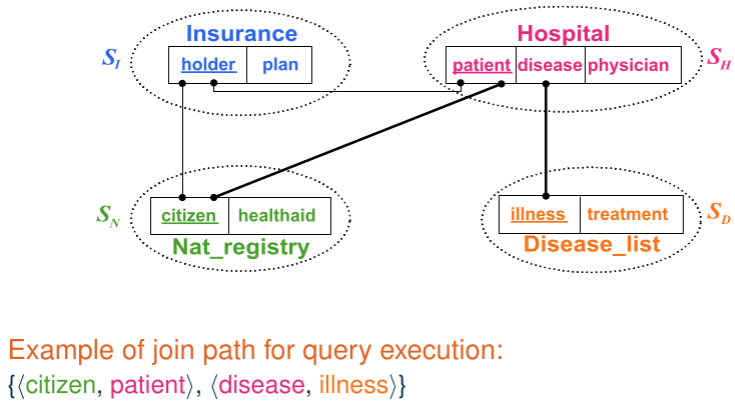
\includegraphics[width=1\linewidth]{images/scenario.png}
\end{figure}


\section{Permessi}
I permessi vengono espressi come una coppia $[Attributes, Join Path] \rightarrow Subject$

$\rightarrow$ \textit{il soggetto è autorizzato ad accedere a tutti gli attributi listati, applicando il join path}

\begin{figure}[H]
    \centering
    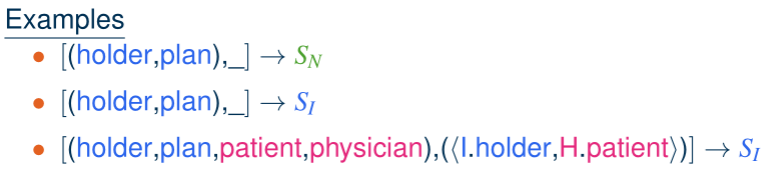
\includegraphics[width=0.8\linewidth]{images/permessi-ex.png}
\end{figure}

\noindent I join path aumentano il potere espressivo, e possono:
\begin{itemize}
    \item Rappresentare \textbf{vincoli di connettività:} stabilisco come sono collegate relazioni diverse
    
    \begin{figure}[H]
        \centering
        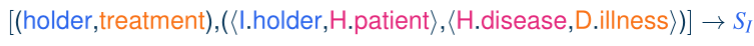
\includegraphics[width=0.8\linewidth]{images/vincoli-conn.png}
    \end{figure}
    \textit{mi dicono come collegare le relazioni affinché questi attributi siano 
    accessibili a un particolare soggetto}
    
    \newpage
    \item Esprimere \textbf{restrizioni sulla quantità di informazioni} a cui un soggetto può accedere 
    
    \begin{figure}[H]
        \centering
        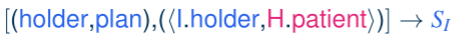
\includegraphics[width=0.5\linewidth]{images/restrizioni.png}
    \end{figure}

    \textit{posso accedere solo alle tuple blu che si uniscono in join alla relazione rosa}

\end{itemize}

\noindent Bisogna fare attenzione al fatto che:
\begin{itemize}
    \item un rilascio di meno tuple (dovuto ad un join path restrittivo) 
    non implica per forza un rilascio di meno informazion
    \begin{figure}[H]
        \centering
        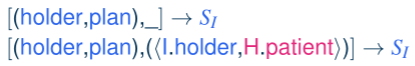
\includegraphics[width=0.5\linewidth]{images/ex1.png}
    \end{figure}
    \item può essere inutile se coinvolge i vincoli di integrità referenziale
    \begin{figure}[H]
        \centering
        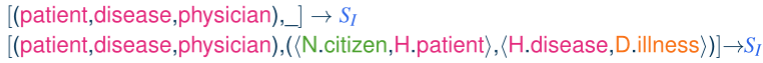
\includegraphics[width=0.9\linewidth]{images/ex2.png}
    \end{figure}
\end{itemize} 

\section{Profilo della relazione}
È un concetto che cerca di catturare il concetto di informazione aggiuntiva non esplicita;
il \textbf{profilo di una relazione} è una tripla $[R^\pi, R^{\bowtie}, R^\sigma]$, dove:
\begin{itemize}
    \item $R^\pi$ è la relazione esplicita
    \item $R^{\bowtie}$ è il join path eseguito per ottenere la relazione $R$
    \begin{itemize}
        \item \textit{come ho ottenuto questa relazione? è stata ottenuta da un join?}
    \end{itemize}
    \item $R^\sigma$ è il set di attributi che sono stati coinvolti in operazioni di selezioni 
    applicate per ottenere la relazione $R$
    \begin{itemize}
        \item \textit{R deriva da qualche condizione applicata su attributi che non sono esplicitamente presenti nella relazione?}
    \end{itemize}
\end{itemize}

\subsubsection{Esempio}

\begin{figure}[H]
    \centering
    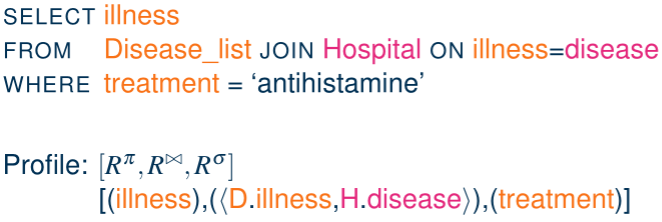
\includegraphics[width=0.7\linewidth]{images/relation-profile-ex.png}
\end{figure}

\section{Vista autorizzata}

Un soggetto $S$ è autorizzato ad accedere ad una vista $R$ sse:

\noindent \hl{ $\exists [Attributes, Join Path]
\rightarrow S | R^\pi \cup R^\sigma \subseteq Attributes AND R^{\bowtie} = Join Path$}

\noindent $\Rightarrow$ \textit{Un soggeto è autorizzato ad accedere ad una relazione quando:
\begin{itemize}
    \item tutti gli attributi espliciti e quelli che usati per definere le condizioni che hanno 
    ristretto le tuple che fanno parte della relazione, sono attributi a cui il soggetto può accedere
    \item il join nella componente R deve essere uguale al join path a cui il soggetto è autorizzato; devono essere ottenuti in quel 
    modo, altrimenti sta accedendo ad informazioni a cui non ha diritto ad accedere
\end{itemize}
}

\begin{figure}[H]
    \centering
    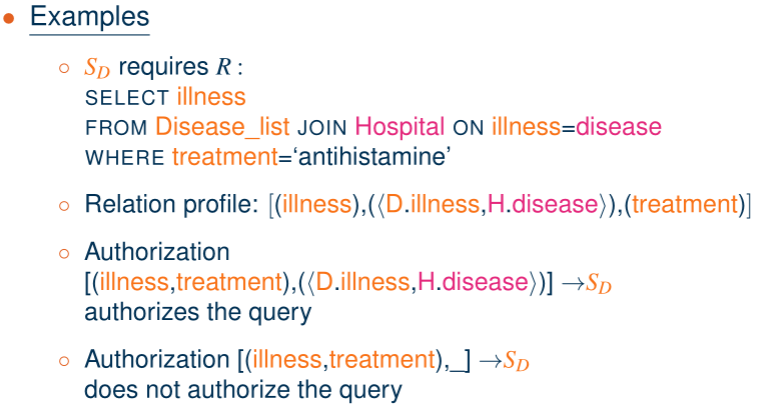
\includegraphics[width=0.8\linewidth]{images/auth-view-ex.png}
\end{figure}

\section{Rilasci autorizzati}
Devo trovare un modo per eseguire la computazione in modo che rispetti i vincoli del sistema.
Le operazioni si dividono in:
\begin{itemize}
    \item \textbf{Unarie}; possono essere eseguite dal server $S$ che tiene la relazione
    \begin{itemize}
        \item proiezione: $\pi_X(R)$
        \item selezione: $\sigma_X(R)$
    \end{itemize}
    \item Operazioni di \textbf{join}; possono essere eseguite solo se implicano il rilascio 
    di \textit{viste autorizzate}. Si possono usare due strategie per eseguire il join soddisfando le autorizzazioni:
    \begin{itemize}
        \item Regular join (master e slave) 
        \begin{figure}[H]
            \centering
            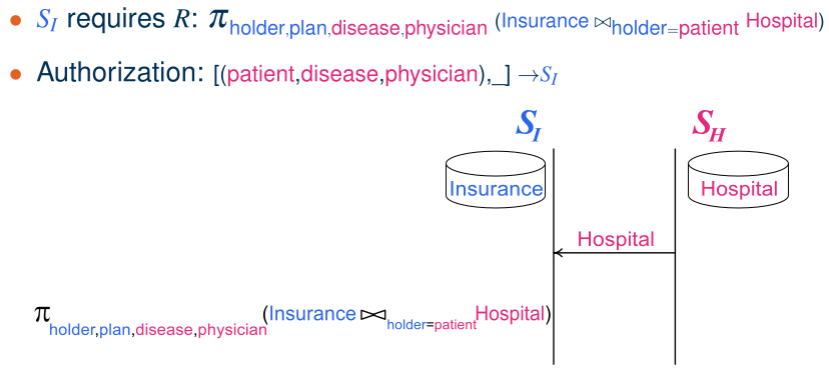
\includegraphics[width=1\linewidth]{images/regular-join.png}
        \end{figure}

        \item Semi-join
        \begin{figure}[H]
            \centering
            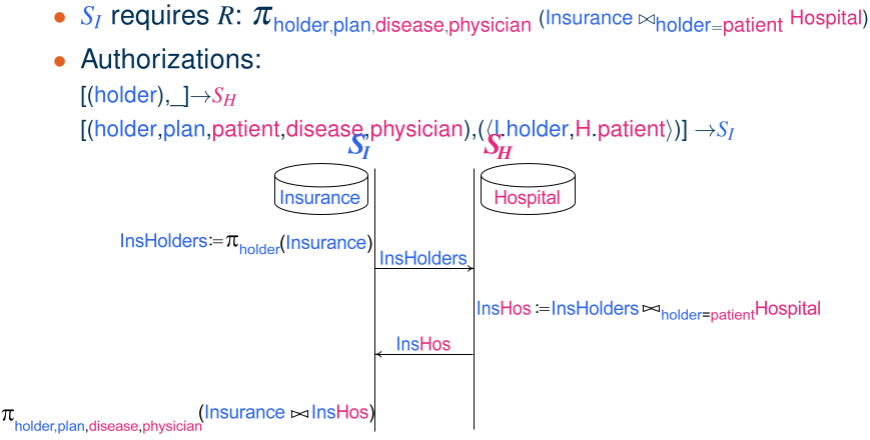
\includegraphics[width=1\linewidth]{images/semi-join.png}
        \end{figure}
    \end{itemize}
 \end{itemize}


\section{Algoritmo}
Data la computazione che voglio eseguire e dato l'insieme di autorizzazioni, l'obiettivo 
è quello di calcolare come eseguire la computazione in modo da rispettare le autorizzazioni.

\noindent L'idea è di fare l'assegnamento in due passi:
\begin{enumerate}
    \item Cerco tutti i soggetti che sono potenzialmente autorizzati ad eseguire una operazione 
    \begin{itemize}
        \item faccio una visita post-order dell'albero (L, R, root; in pratica dalle foglie risalgo) 
    \end{itemize}
    \item Faccio una visita in pre-order dell'albero e ne scelgo uno; può essere fatta in diversi modi in base a qual è il parametro di voglio ottimizzare
\end{enumerate}














\end{document}
